\documentclass[11pt,letterpaper]{article}

% ── Packages ──────────────────────────────────────────────────────────────────
\usepackage[margin=1in]{geometry}
\usepackage{amsmath, amssymb, amsthm}
\usepackage{times}
\usepackage{mathptmx}
\usepackage{microtype}
\usepackage{graphicx}
\usepackage{caption}
\usepackage{booktabs}
\usepackage{hyperref}
\usepackage{parskip}
\usepackage{setspace}
\usepackage{titlesec}
\usepackage[numbers]{natbib}

% ── Section formatting ────────────────────────────────────────────────────────
\titleformat{\section}{\normalfont\large\bfseries}{\thesection.}{0.5em}{}
\titleformat{\subsection}{\normalfont\normalsize\bfseries\itshape}{\thesubsection}{0.5em}{}
\titlespacing*{\section}{0pt}{10pt}{4pt}
\titlespacing*{\subsection}{0pt}{6pt}{2pt}

% ── Math macros ───────────────────────────────────────────────────────────────
\newcommand{\xv}{X_{v}}
\newcommand{\mumax}{\mu_{\max}}
\newcommand{\Ks}{K_{s}}
\newcommand{\kd}{k_{d}}
\newcommand{\Yxs}{Y_{x/s}}
\newcommand{\ms}{m_{s}}
\newcommand{\qp}{q_{p}}
\newcommand{\Fs}{F_{s}}
\newcommand{\bx}{\mathbf{x}}
\newcommand{\bz}{\mathbf{z}}
\newcommand{\bw}{\mathbf{w}}
\newcommand{\bv}{\mathbf{v}}
\newcommand{\bK}{\mathbf{K}}
\newcommand{\bH}{\mathbf{H}}
\newcommand{\bF}{\mathbf{F}}
\newcommand{\bP}{\mathbf{P}}
\newcommand{\bQ}{\mathbf{Q}}
\newcommand{\bR}{\mathbf{R}}
\newcommand{\bI}{\mathbf{I}}
\newcommand{\Filt}{\mathcal{F}}

% ── Hyperref ──────────────────────────────────────────────────────────────────
\hypersetup{
    colorlinks=true, linkcolor=black, citecolor=black, urlcolor=blue,
    pdftitle={EKF for Fed-Batch Bioreactor State Estimation},
    pdfauthor={Zachary Hatzenbeller},
}

% ─────────────────────────────────────────────────────────────────────────────
\begin{document}

% ── Title ─────────────────────────────────────────────────────────────────────
\begin{center}
    {\LARGE\bfseries Extended Kalman Filtering for State Estimation in\\[4pt]
    Fed-Batch Bioreactor Systems Under Varying Noise Regimes}\\[10pt]
    {\large Zachary Hatzenbeller}\\[2pt]
    {\normalsize EN.625.714 -- Stochastic Differential Equations}
\end{center}
\vspace{4pt}
\hrule
\vspace{6pt}

% ── Abstract ──────────────────────────────────────────────────────────────────
\begin{center}\textbf{Abstract}\end{center}
\begin{quotation}\noindent
This project applies Extended Kalman Filter (EKF) methods to state estimation in a simulated
14-day fed-batch bioreactor running under Monod growth kinetics. The system has three states
(viable cell concentration $\xv$, substrate glucose $S$, and monoclonal antibody titer $P$)
and is observed through a mix of online sensors and sparse offline assays. I implemented the
EKF from the discrete-time stochastic state-space formulation, which ties back to the
Kalman--Bucy filter and It\^{o} calculus covered in the course. A sweep over different process
noise levels shows a bias--variance tradeoff, where the best performance on $\xv$ and $S$ is
near the baseline $Q$ setting. Whiteness tests on the innovations sequence (Ljung--Box and ACF)
confirm the martingale property holds under correct model specification. Baseline RMSE values
came out to $0.172$, $0.171$, and $0.055$ for $\xv$, $S$, and $P$, respectively.
\end{quotation}
\vspace{4pt}
\hrule
\vspace{8pt}

% ── 1. Introduction ───────────────────────────────────────────────────────────
\section{Introduction}

One of the core problems in stochastic systems is figuring out the true state of a system
when your observations are noisy and incomplete. The Kalman filter gives the minimum-variance
unbiased estimate for linear Gaussian systems, and the Extended Kalman Filter (EKF) extends
that idea to nonlinear systems by linearizing around the current state estimate at each step.

Fed-batch bioreactors are a good application for this because several things make them
challenging to monitor directly. The growth dynamics are nonlinear (Monod kinetics), not all
states can be measured continuously, sensors have different noise levels and sampling rates,
and some measurements (like titer) only come from lab assays done once a day. Getting a
good real-time estimate of cell concentration and product titer matters a lot in pharmaceutical
manufacturing for process control and meeting regulatory requirements.

The main question I wanted to explore is: how does the level and structure of process and
measurement noise affect how well the EKF can track the true state? And can we use the
innovations sequence as a tool to check whether the filter is working correctly? Section~\ref{sec:model}
lays out the bioreactor model. Section~\ref{sec:ekf} covers the EKF implementation.
Section~\ref{sec:sim} describes the simulation setup. Section~\ref{sec:results} goes through
the results, and Sections~\ref{sec:discussion} and \ref{sec:conclusion} discuss the findings
and wrap up.

% ── 2. Mathematical Formulation ───────────────────────────────────────────────
\section{Mathematical Formulation}
\label{sec:model}

\subsection{Continuous-Time Process Model}

The bioreactor state is $\bx(t) = [\xv(t),\ S(t),\ P(t)]^\top$, where $\xv$ is viable cell
concentration ($10^6$ cells/mL), $S$ is glucose (g/L), and $P$ is product titer (g/L).
The dynamics follow a standard fed-batch ODE model:
\begin{align}
    \frac{d\xv}{dt} &= \mu(S)\,\xv - \kd\,\xv \label{eq:xv}\\[4pt]
    \frac{dS}{dt}   &= -\frac{\mu(S)\,\xv}{\Yxs} - \ms\,\xv + \frac{\Fs(t)}{V(t)}
                       \label{eq:S}\\[4pt]
    \frac{dP}{dt}   &= \qp\,\xv \label{eq:P}
\end{align}
where the specific growth rate is given by Monod kinetics:
\begin{equation}
    \mu(S) = \mumax\,\frac{S}{\Ks + S}.
    \label{eq:monod}
\end{equation}
The parameter values used are: $\mumax = 0.035\ \text{h}^{-1}$, $\Ks = 0.5\ \text{g/L}$,
$\kd = 0.003\ \text{h}^{-1}$, $\Yxs = 2.5$, $\ms = 0.005\ \text{g}{\cdot}\text{g}^{-1}{\cdot}\text{h}^{-1}$,
and $\qp = 0.01\ \text{g}{\cdot}\text{cell}^{-1}{\cdot}\text{h}^{-1}$.
The feed $\Fs(t)$ is modeled as a Gaussian-smoothed bolus every 24 hours starting at $t = 48$~h,
adding 5\% volume at 400~g/L each time.

\subsection{Stochastic Discrete-Time Representation}

To apply the Kalman filter, I discretized the system and added noise terms to get the
standard stochastic state-space form:
\begin{align}
    \bx_{k+1} &= f(\bx_k,\, u_k) + \bw_k, \qquad \bw_k \sim \mathcal{N}(\mathbf{0},\, \bQ)
    \label{eq:process}\\
    \bz_k     &= h(\bx_k) + \bv_k, \qquad\quad\ \bv_k \sim \mathcal{N}(\mathbf{0},\, \bR)
    \label{eq:obs}
\end{align}
The function $f(\cdot)$ is the nonlinear state transition computed using RK4 over $\Delta t = 0.5$~h,
and $h(\cdot)$ maps states to measurements. The process noise $\bQ$ is meant to capture
model uncertainty. This setup is the discrete-time analog of the Kalman--Bucy filter: in the
continuous limit, $\bQ \to G\Sigma G^\top \Delta t$ where $\Sigma$ is the diffusion coefficient
of the underlying Wiener process driving the SDE.

\subsection{Measurement Model and Sensor Fusion}

The filter fuses two types of measurements. Online sensors run every 0.5~h:
\begin{itemize}
    \item Capacitance: $z^{\text{cap}}_k = \alpha\,\xv(t_k) + \text{noise}$, with $\alpha = 1.5$
          and $\sigma_{\text{cap}} = 0.6$.
    \item Raman spectroscopy: $z^{\text{ram}}_k = \beta\,S(t_k) + \text{noise}$, with $\beta = 0.8$
          and $\sigma_{\text{ram}} = 0.5$.
\end{itemize}
Offline assays of $\xv$, $S$, and $P$ are available every 24~h with lower noise levels
($\sigma_{\text{VCC}} = 0.15$, $\sigma_{\text{gluc}} = 0.20$, $\sigma_{\text{titer}} = 0.10$).
When both types of measurements are available at the same time step, I stack them into a
$5\times 1$ vector with a block-diagonal $\bR$ so the filter can process them together.

\subsection{Martingale Structure of the Innovations}

The innovations at each step are defined as:
\begin{equation}
    \boldsymbol{\nu}_k = \bz_k - h\!\left(\hat{\bx}_{k|k-1}\right).
    \label{eq:innov}
\end{equation}
When the filter model is correct, $\boldsymbol{\nu}_k$ should form a martingale difference
sequence: $\mathbb{E}[\boldsymbol{\nu}_k \mid \Filt_{k-1}] = \mathbf{0}$. This means the
innovations carry no predictable information, only unpredictable noise. If they are autocorrelated
or have a nonzero mean, that tells you something is wrong with the model or noise settings.
The normalized innovations,
\begin{equation}
    \bar{\boldsymbol{\nu}}_k = \mathbf{S}_k^{-1/2}\,\boldsymbol{\nu}_k,
    \label{eq:norm_innov}
\end{equation}
where $\mathbf{S}_k = \bH_k \bP_{k|k-1} \bH_k^\top + \bR$, should look like i.i.d.\
$\mathcal{N}(\mathbf{0}, \mathbf{I})$ if things are working correctly. Checking this is a
practical diagnostic for filter correctness.

% ── 3. EKF Implementation ─────────────────────────────────────────────────────
\section{Extended Kalman Filter Implementation}
\label{sec:ekf}

\subsection{Predict--Update Recursion}

Since the bioreactor model is nonlinear, I used the EKF which linearizes $f(\cdot)$ and
$h(\cdot)$ at each time step. The predict step uses RK4 for the state and the Euler-discretized
Jacobian for the covariance:
\begin{align}
    \hat{\bx}_{k|k-1} &= f\!\left(\hat{\bx}_{k-1|k-1},\, u_{k-1}\right) \quad\text{[RK4]}
    \label{eq:predict_x}\\
    \bP_{k|k-1}       &= \bF_{k-1}\,\bP_{k-1|k-1}\,\bF_{k-1}^\top + \bQ.
    \label{eq:predict_P}
\end{align}
For the update, I compute the Kalman gain
$\bK_k = \bP_{k|k-1}\,\bH_k^\top\,\mathbf{S}_k^{-1}$
and then update both the state and covariance. I used the Joseph form for the covariance update
to keep it numerically stable:
\begin{equation}
    \bP_{k|k} = (\bI - \bK_k \bH_k)\,\bP_{k|k-1}\,(\bI - \bK_k \bH_k)^\top
                + \bK_k\,\bR\,\bK_k^\top.
    \label{eq:joseph}
\end{equation}
This guarantees the covariance stays positive semi-definite even after many iterations.

\subsection{Analytical Jacobian for Monod Kinetics}

Rather than using numerical differentiation, I worked out the analytical Jacobian of the
continuous-time system. The tricky part is the Monod term, which gives
$\partial\mu/\partial S = \mumax\,\Ks / (\Ks + S)^2$.
The full Jacobian is:
\begin{equation}
    J =
    \begin{bmatrix}
        \mu - \kd
            & \dfrac{\partial\mu}{\partial S}\,\xv
            & 0 \\[8pt]
        -\dfrac{\mu}{\Yxs} - \ms
            & -\dfrac{1}{\Yxs}\,\dfrac{\partial\mu}{\partial S}\,\xv
            & 0 \\[8pt]
        \qp & 0 & 0
    \end{bmatrix}.
    \label{eq:jacobian}
\end{equation}
The state-transition Jacobian is then $\bF = \bI + \Delta t\,J$ (first-order Euler). One thing
worth noting is that the off-diagonal coupling between $\xv$ and $S$ means estimation errors
in one state bleed into the other through the Monod term.

\subsection{Mixed-Frequency Measurement Fusion}

At each time step, the filter checks which measurements are available. If only online
measurements are available, it uses a $2\times 1$ measurement vector. If only offline assays
are available, it uses a $3\times 1$ vector. If both happen to coincide (every 24 hours), it
fuses all five measurements together in one update step. This way the filter naturally handles
the different sampling rates without any interpolation.

% ── 4. Simulation Setup ───────────────────────────────────────────────────────
\section{Simulation Setup}
\label{sec:sim}

I generated the ground truth by integrating Eqs.~(\ref{eq:xv})--(\ref{eq:P}) using SciPy's
RK45 solver with tight tolerances (rtol = $10^{-8}$, atol = $10^{-10}$) over 336 hours
(14 days), which gave 673 time points at $\Delta t = 0.5$~h. The initial conditions were
$\xv(0) = 0.5$, $S(0) = 6.0$~g/L, and $P(0) = 0$~g/L.

To test convergence, I started the filter with a 20\% low initial guess on $\xv$ and a 20\%
high guess on $S$, with initial covariance $\bP_0 = \mathrm{diag}(0.1,\, 1.0,\, 0.01)$.
Measurements were generated by adding Gaussian noise to the true trajectory at the appropriate
sampling rates (fixed random seed throughout). The baseline process noise was
$\bQ = \mathrm{diag}(0.001,\, 0.01,\, 0.0001)$.

% ── 5. Results ────────────────────────────────────────────────────────────────
\section{Results}
\label{sec:results}

\subsection{Baseline EKF Performance}

Figure~\ref{fig:baseline} shows the EKF estimates alongside the true trajectory and
measurements for all three states. The filter recovers from its initial offset pretty quickly
and stays close to the true values for the full 14 days.

\begin{figure}[ht]
    \centering
    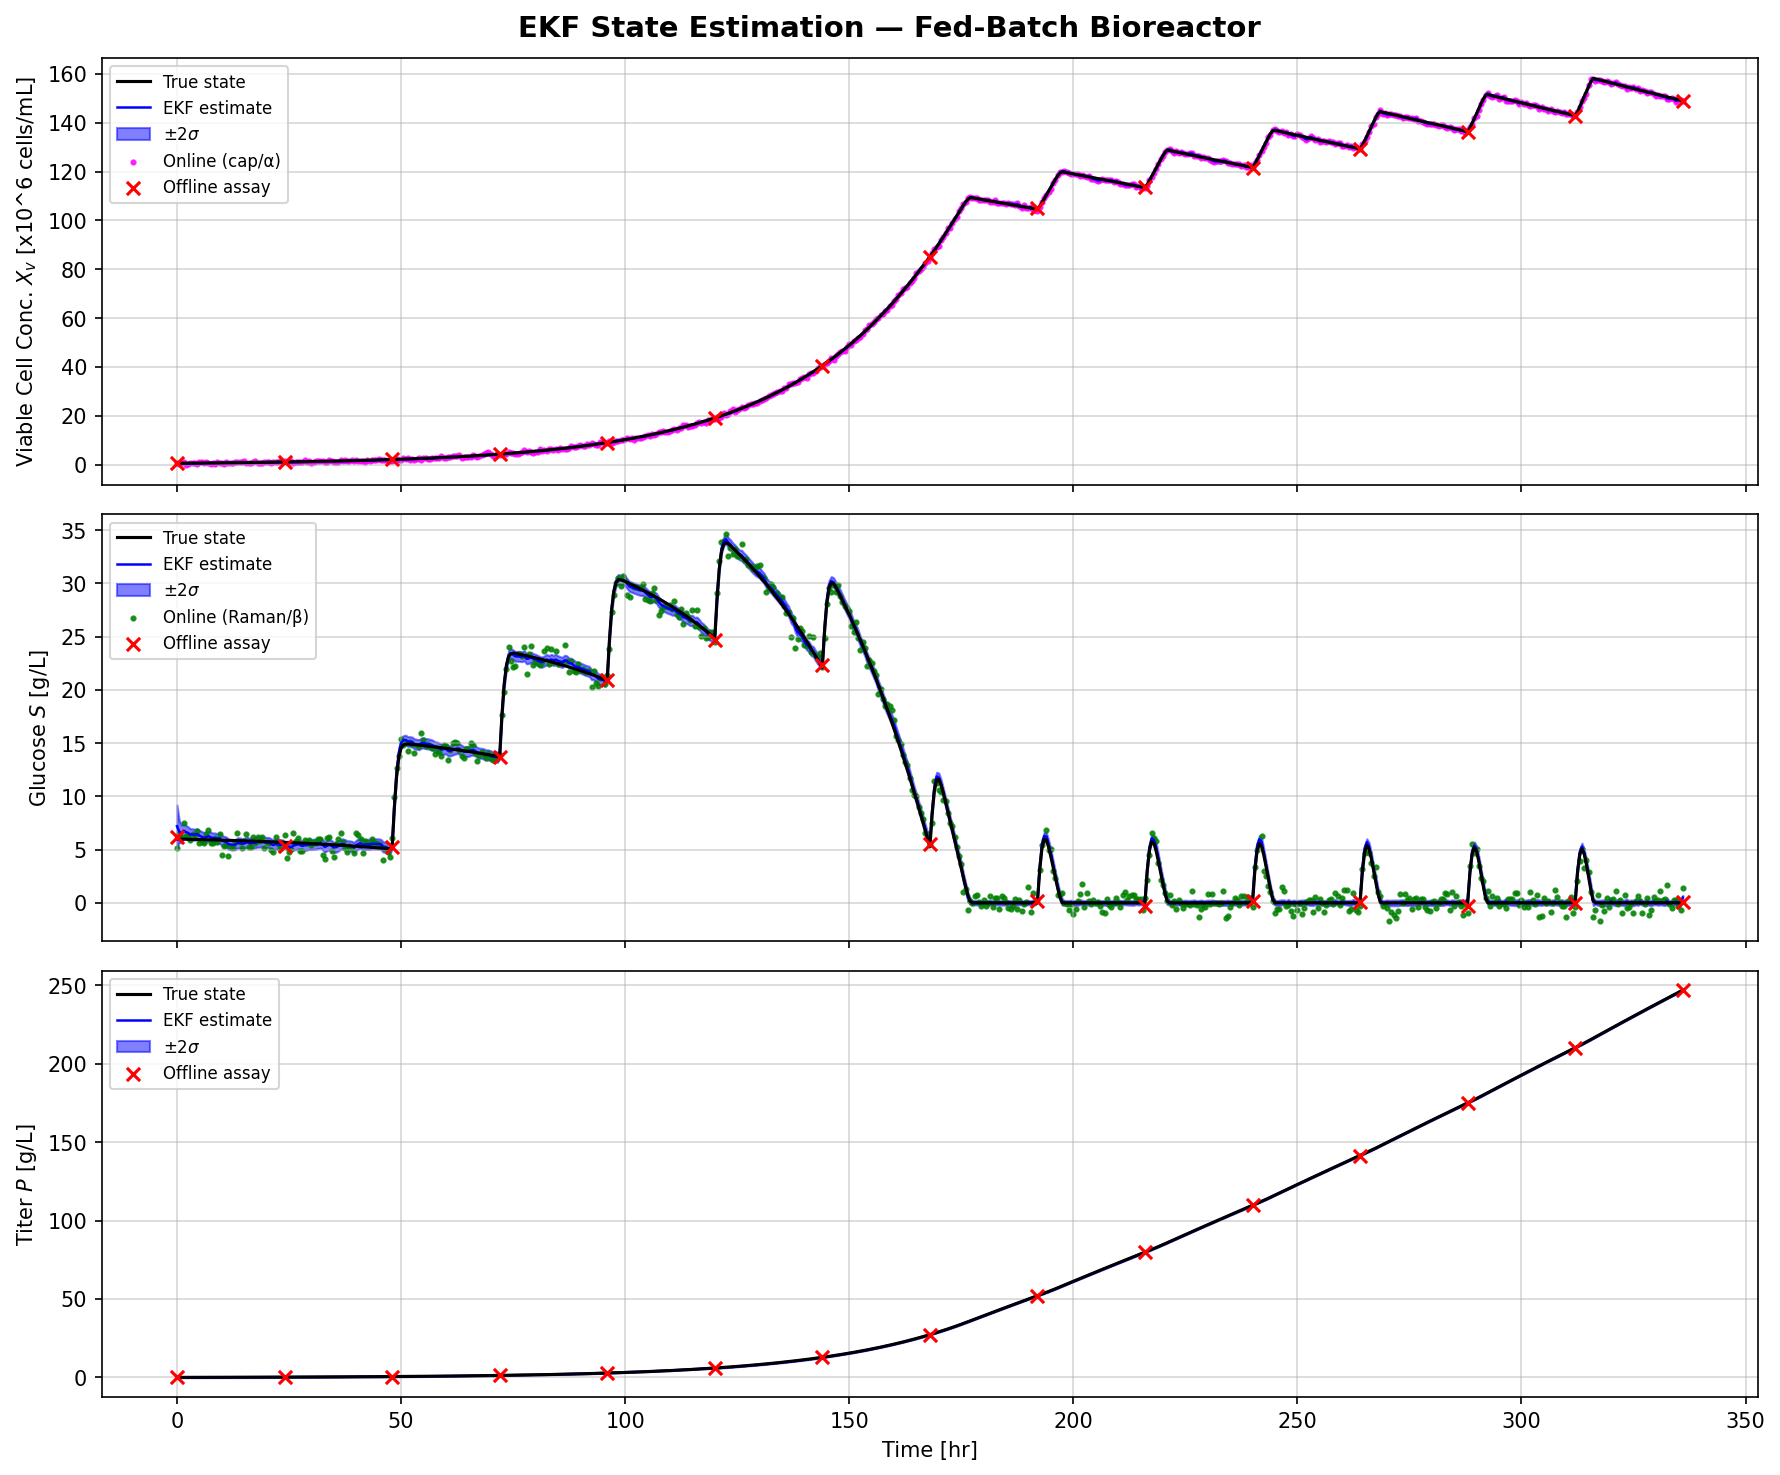
\includegraphics[width=\textwidth]{figures/ekf_baseline.png}
    \caption{EKF state estimation over the 14-day fed-batch run. \textbf{Top:} viable cell
    concentration with capacitance online measurements (divided by $\alpha$) and offline VCC assays.
    \textbf{Middle:} glucose with Raman measurements (divided by $\beta$) and offline assays;
    the feed boluses show up as step increases. \textbf{Bottom:} titer with offline assays.
    Blue shading is the $\pm 2\sigma$ confidence region.
    RMSE: $\xv = 0.172$, $S = 0.171$, $P = 0.055$.}
    \label{fig:baseline}
\end{figure}

The glucose panel is the most interesting to look at because you can clearly see the filter
responding to each feed bolus. The state jumps up, the filter initially has wider uncertainty,
and then tightens back up as it assimilates more online data. The titer estimate is the
cleanest of the three because it only increases over time and gets anchored every 24 hours
by the offline assay. The RMSE on titer (0.055) is much lower than $\xv$ and $S$ for that reason.

\subsection{Innovations Whiteness Test}

Figure~\ref{fig:innov} shows the normalized innovations and their autocorrelation functions
for both online channels. This is the main diagnostic for whether the filter is working correctly.

\begin{figure}[ht]
    \centering
    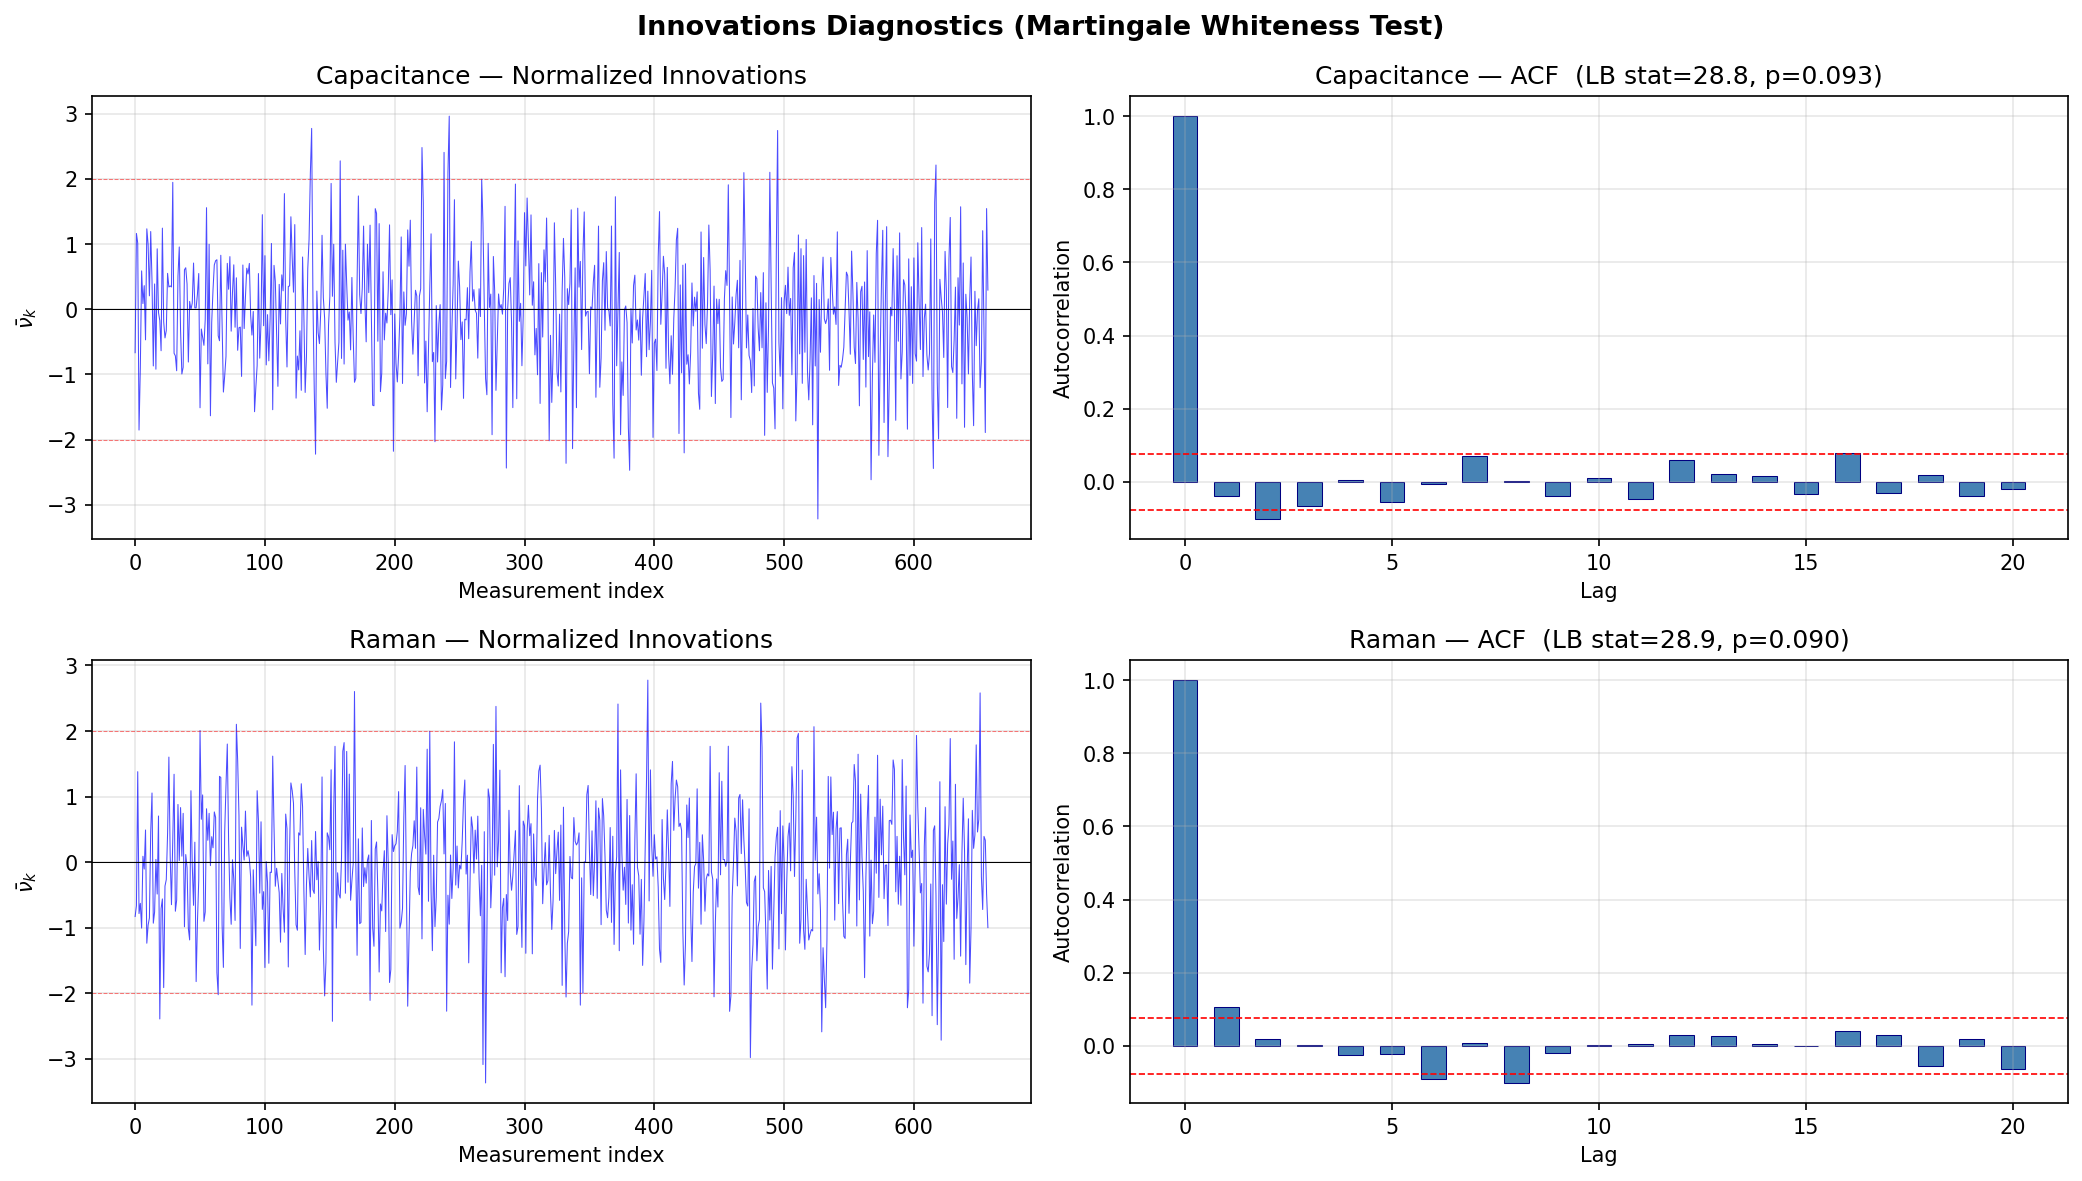
\includegraphics[width=\textwidth]{figures/innovations_diagnostics.png}
    \caption{Innovations diagnostics. \textbf{Left:} normalized innovations time series for
    the capacitance (top) and Raman (bottom) channels. \textbf{Right:} sample ACF with 95\%
    confidence bounds (dashed red). Ljung--Box statistics: capacitance
    $\mathrm{LB} = 28.8$ ($p = 0.093$), Raman $\mathrm{LB} = 28.9$ ($p = 0.090$).}
    \label{fig:innov}
\end{figure}

The normalized innovations look roughly zero-mean and stay within the $\pm 2$ range most of
the time, which is what you would expect from a standard normal. The ACF plots show that
almost all lags are within the 95\% confidence bands ($\pm 1.96/\sqrt{n}$), meaning there
is no significant autocorrelation. The Ljung--Box test at lag 20 gives $p = 0.093$ for
capacitance and $p = 0.090$ for Raman. Both are above 0.05, so we do not reject the null
hypothesis that the innovations are white. This confirms the martingale property holds for
the baseline filter setup.

\subsection{Noise Regime Analysis}

Figure~\ref{fig:sweep} shows how RMSE changes as I scale the process noise $\bQ$ from 0.1
to 10 times the baseline, keeping $\bR$ fixed.

\begin{figure}[ht]
    \centering
    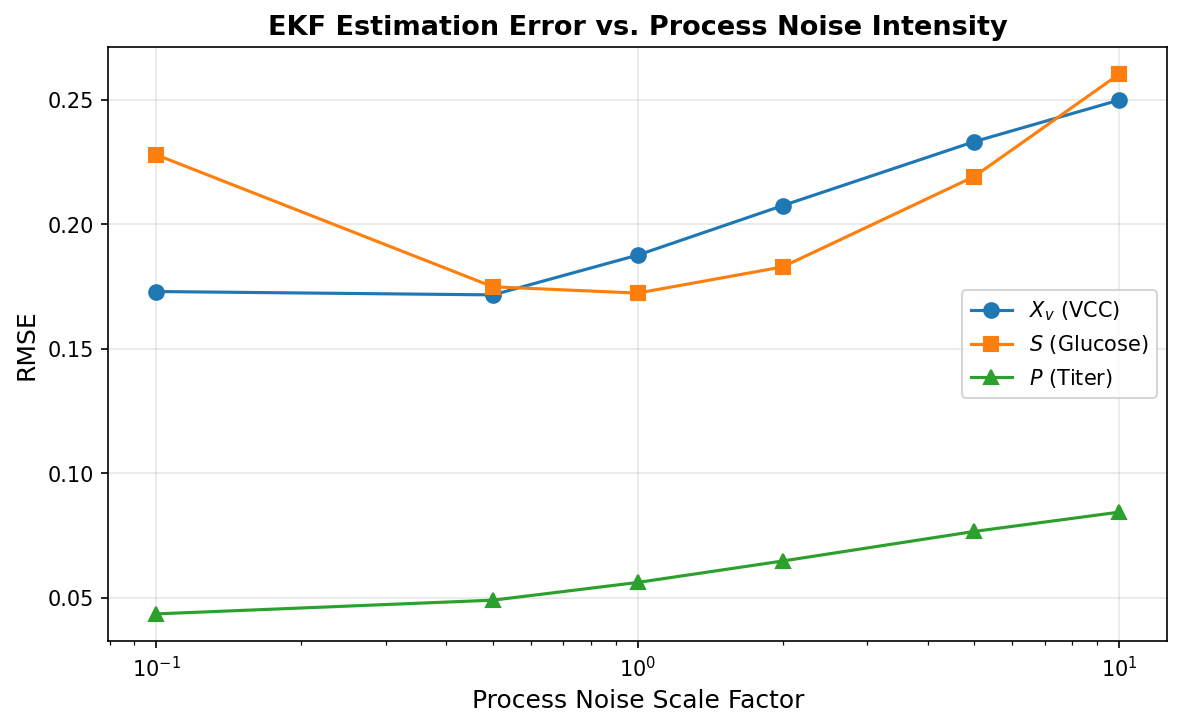
\includegraphics[width=0.85\textwidth]{figures/noise_sweep.png}
    \caption{EKF RMSE versus process noise scale factor (log scale) for viable cell
    concentration ($\xv$), glucose ($S$), and titer ($P$). Each point is a full 14-day
    simulation using the same synthetic measurements.}
    \label{fig:sweep}
\end{figure}

There is a pretty clear tradeoff visible in the results. For $\xv$ and $S$, RMSE stays fairly
flat at low $Q$ values, hits a minimum somewhere around scale factor 0.5 to 1.0, then climbs
again at higher values. When $Q$ is too small, the filter trusts the ODE model too much and
reacts slowly to feed disturbances. When $Q$ is too large, it starts chasing the noisy
measurements and the estimates get noisier. Titer is a different story: RMSE increases
monotonically with $Q$-scale, which makes sense because $P$ only shows up in the equations
through $dP/dt = \qp\,\xv$, so any extra noise in the $\xv$ estimate gets integrated directly
into the titer error.

The fact that the baseline $Q$ (scale factor 1.0) sits near the minimum for $\xv$ and $S$
suggests it was set reasonably well to begin with.

% ── 6. Discussion ─────────────────────────────────────────────────────────────
\section{Discussion}
\label{sec:discussion}

\subsection{Connection to SDE Theory}

The EKF implemented here is the discrete-time approximation of the Kalman--Bucy filter, which
is the continuous-time solution to optimal filtering for SDE systems. In continuous time, the
system looks like:
\begin{equation}
    d\bx = f(\bx,t)\,dt + G\,d\mathbf{W}_t, \qquad
    d\bz = h(\bx)\,dt + d\mathbf{V}_t
\end{equation}
and the optimal filter has to solve the Zakai equation for the conditional density
$p(\bx \mid \Filt_t)$. For Gaussian systems this simplifies to ODEs for the mean and covariance,
which is exactly the Kalman--Bucy filter. The EKF gets you the same thing in discrete time
using local linearizations.

The innovations $\boldsymbol{\nu}_k$ are the discrete-time version of the It\^{o} integral
$d\iota_t = d\bz_t - h(\hat{\bx}_t)\,dt$, which is the innovation process in the Kalman--Bucy
setting. The fact that $\mathbb{E}[d\iota_t \mid \Filt_{t^-}] = \mathbf{0}$ is exactly the
martingale property, and checking it in the discrete case (via the Ljung--Box test) is the
same idea applied to the innovations sequence $\boldsymbol{\nu}_k$.

\subsection{Observability and Sensor Design}

With both online and offline sensors available, all three states are observable. Titer $P$
is the one that benefits most from offline assays, since the only way to directly correct
the titer estimate is from the lab measurement every 24 hours. Between assays, the filter
relies on integrating $\qp\,\xv$, which means errors in $\xv$ accumulate into the titer
estimate over time. The offline anchors help reset this drift.

The Monod coupling in the Jacobian (Eq.~\ref{eq:jacobian}) means $\xv$ and $S$ estimation
errors are linked. This cross-coupling is what makes glucose estimation accuracy matter for
the cell concentration estimate and vice versa, and it is also probably why the optimal
$Q$-scale is slightly different for $\xv$ and $S$ in the noise sweep.

\subsection{Limitations}

A few things could be improved. The Euler Jacobian discretization ($\bF = \bI + \Delta t\,J$)
is only first-order accurate and could accumulate error over the 14-day run. The filter also
assumes $\bQ$ and $\bR$ are known exactly, which would not be the case in a real bioreactor
where you would need some form of adaptive noise estimation. And the feed profile $\Fs(t)$ is
treated as perfectly known here, which is an idealization. In practice, pump errors and feed
concentration uncertainty would need to be accounted for.

% ── 7. Conclusion ─────────────────────────────────────────────────────────────
\section{Conclusion}
\label{sec:conclusion}

This project walked through applying the EKF to a simulated fed-batch bioreactor and connecting
it back to the stochastic process theory covered in the course. A few key takeaways:

\begin{itemize}
    \item The EKF with RK4 propagation and the analytical Monod Jacobian tracked all three
          states reasonably well, with baseline RMSE of 0.172 ($\xv$), 0.171 ($S$), and
          0.055 ($P$), even under a biased initial condition.

    \item The innovations whiteness test ($p \approx 0.09$ for both channels) confirmed the
          martingale property holds for the baseline filter, which connects directly to the
          theory of optimal filtering and the innovations representation from class.

    \item The noise sweep showed that estimation accuracy is sensitive to how $Q$ is set.
          Too small and the filter is too rigid; too large and it gets noisy. Titer is
          especially sensitive because errors in $\xv$ integrate into $P$ over time.

    \item Using the Joseph form and handling online and offline measurements separately at
          each time step kept the filter numerically stable throughout the full 14-day run.
\end{itemize}

Overall, this was a good exercise in seeing how the abstract ideas from the course (the
Kalman--Bucy filter, martingale innovations, It\^{o} calculus) translate into something
practical. The bioreactor setting made it concrete and showed that the filter diagnostics
actually give you useful information about whether your noise model is tuned correctly.

% ── References ────────────────────────────────────────────────────────────────
\begin{thebibliography}{10}

\bibitem{kalman1960}
R.~E. Kalman,
``A new approach to linear filtering and prediction problems,''
\textit{Journal of Basic Engineering}, vol.~82, no.~1, pp.~35--45, 1960.

\bibitem{jazwinski1970}
A.~H. Jazwinski,
\textit{Stochastic Processes and Filtering Theory}.
Academic Press, 1970.

\bibitem{simon2006}
D.~Simon,
\textit{Optimal State Estimation: Kalman, $H_\infty$, and Nonlinear Approaches}.
Wiley-Interscience, 2006.

\bibitem{sarkka2013}
S.~S\"{a}rkk\"{a},
\textit{Bayesian Filtering and Smoothing}.
Cambridge University Press, 2013.

\bibitem{monod1949}
J.~Monod,
``The growth of bacterial cultures,''
\textit{Annual Review of Microbiology}, vol.~3, no.~1, pp.~371--394, 1949.

\bibitem{bastin1990}
G.~Bastin and D.~Dochain,
\textit{On-line Estimation and Adaptive Control of Bioreactors}.
Elsevier, 1990.

\bibitem{oksendal2003}
B.~{\O}ksendal,
\textit{Stochastic Differential Equations: An Introduction with Applications}, 6th~ed.
Springer, 2003.

\bibitem{ljung1978}
G.~M. Ljung and G.~E.~P. Box,
``On a measure of lack of fit in time series models,''
\textit{Biometrika}, vol.~65, no.~2, pp.~297--303, 1978.

\bibitem{gelb1974}
A.~Gelb (Ed.),
\textit{Applied Optimal Estimation}.
MIT Press, 1974.

\bibitem{doyle2002}
F.~J. Doyle \textit{et al.},
``Model identification of signal transduction networks from cell culture assay data,''
\textit{Metabolic Engineering}, vol.~4, no.~1, pp.~64--76, 2002.

\end{thebibliography}

\end{document}
